% !TEX root = ../MA119-Question-Bank.tex




% \pgfmathtruncatemacro{\a}{random(1,5)}
% \pgfmathtruncatemacro{\k}{\a^2}

% \pgfmathdeclarerandomlist{diffone}{{2}{3}{4}{5}}
% \pgfmathdeclarerandomlist{difftwo}{{1}{3}{4}{5}}
% \pgfmathdeclarerandomlist{diffthree}{{1}{2}{4}{5}}
% \pgfmathdeclarerandomlist{difffour}{{1}{2}{3}{5}}
% \pgfmathdeclarerandomlist{difffive}{{1}{2}{3}{4}}

% \ifcase\a\relax%
%   \or \pgfmathrandomitem{\h}{diffone}
%   \or \pgfmathrandomitem{\h}{difftwo}
%   \or \pgfmathrandomitem{\h}{diffthree}
%   \or \pgfmathrandomitem{\h}{difffour}
%   \or \pgfmathrandomitem{\h}{difffive}
%  \fi
%  \edef\h{\h}

\pgfmathtruncatemacro{\a}{random(1,2)}
\pgfmathtruncatemacro{\k}{\a^2}
\pgfmathtruncatemacro{\h}{random(1,3)}
\pgfmathtruncatemacro{\b}{2*\h}
\pgfmathtruncatemacro{\rone}{\h+\a}
\pgfmathtruncatemacro{\rtwo}{\h-\a}
\pgfmathtruncatemacro{\c}{\k-\h^2}


 \mbox{}


\begin{minipage}{\textwidth}
\begin{minipage}{0.6\textwidth}
  Consider the quadratic function
  \[f(x)=-x^2+\b x \ifnum\c=0 \else \constdisplay{\c} \fi.\]
\begin{enumerate}[label={(\arabic*)},afterlabel=\quad, itemindent=0em, wide]
\item Find the line of symmetry.
\item Find the coordinate of the vertex.
\item Find the coordinate of the $y$-intercept.
\item Find the coordinates of the $x$-intercepts.
\item Sketch the graph of the quadratic function.
 % using the information in part A.
\end{enumerate}
\end{minipage}\hspace{-3em}
\begin{minipage}{0.5\textwidth}
\begin{center}
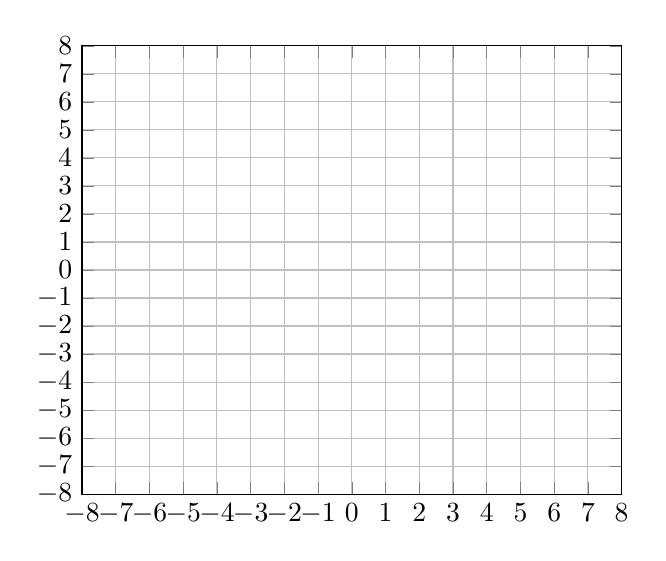
\begin{tikzpicture}[scale=1]
\begin{axis}[
	grid=both,
	ymin=-8,
  ymax=8,
  xmax=8,
  xmin=-8,
  xtick={-8,-7,...,8},
  ytick={-8,-7,...,8},
	% minor tick num=1,
]
  \end{axis}
\end{tikzpicture}
\end{center}
\end{minipage}
\end{minipage}

\begin{solution}

\begin{minipage}{\textwidth}
\begin{minipage}{0.6\textwidth}
\begin{enumerate}[label={(\arabic*)},afterlabel=\quad]
\item The line of symmetry is $x=\h$.
\item The vertex is $(\h, \k)$.
\item The $y$-intercept is $(0, \c)$.
\item The $x$-intercepts are $(\rtwo, 0)$ and $(\rone,0)$.
\item
The graph of $f$ is shown in the right.
\end{enumerate}
\end{minipage}\hspace{-2em}
\begin{minipage}{0.5\textwidth}
\begin{center}
\begin{tikzpicture}[scale=1]
\begin{axis}[
	grid=both,
	ymin=-8,
	ymax=8,
	xmax=8,
	xmin=-8,
	xtick={-8,-7,...,8},
	ytick={-8,-7,...,8},
	% minor tick num=1,
]
 \addplot[thick, samples=100, domain=-2:6]   {-(x-\h)^2+\k};
  \end{axis}
\end{tikzpicture}
\end{center}
\end{minipage}
\end{minipage}
\end{solution}
